% Derived from PGF's shapes.geometric regular-polygon border algorithm.
\documentclass[border=2pt]{standalone}
\usepackage{tikz}
\usetikzlibrary{arrows.meta,shapes.geometric}

\begin{document}
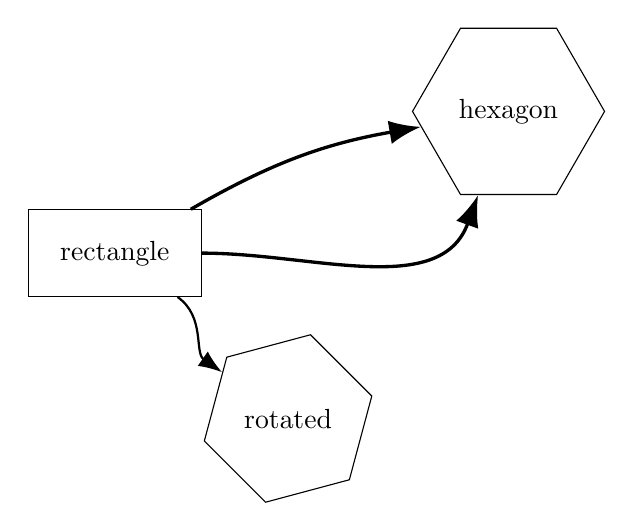
\begin{tikzpicture}[x=1cm,y=1cm]
  \node[draw,rectangle,minimum width=2.2cm,minimum height=1.1cm] (rect) at (0,0) {rectangle};
  \node[draw,regular polygon,regular polygon sides=6,minimum size=1.7cm] (hex) at (5,1.8) {hexagon};
  \node[draw,regular polygon,regular polygon sides=6,regular polygon rotate=15,minimum size=1.35cm] (tilted) at (2.2,-2.1) {rotated};

  \draw[-{Latex[length=4mm,width=3mm]},very thick] (rect) to[out=30,in=190] (hex);
  \draw[{Latex[length=4mm,width=3mm]}-,very thick] (hex) to[out=250,in=0] (rect);
  \draw[-{Latex[length=3mm,width=2.25mm]},thick] (rect) to[out=-35,in=145] (tilted);
\end{tikzpicture}
\end{document}
